\section {ALERTS}

\textit{Alerts} tab displays logged all event of system. Events are collected in two groups:
\begin{itemize}
	\item Errors
	\item Events
\end{itemize}

Group \textit{Errors} contains information about occurred error. Additional we can find out which program and subprogram was runned when error occured and who confirmed error. \\

Button \textit{Clear Errors} is using for clear of current list of error. When any problem still exist, error will be reports again.\\

Group \textit{Events}  contains information about action made by user. There are find out information which parameters of machine has been changed by user.

	\begin{figure}[!h] 
	\centering 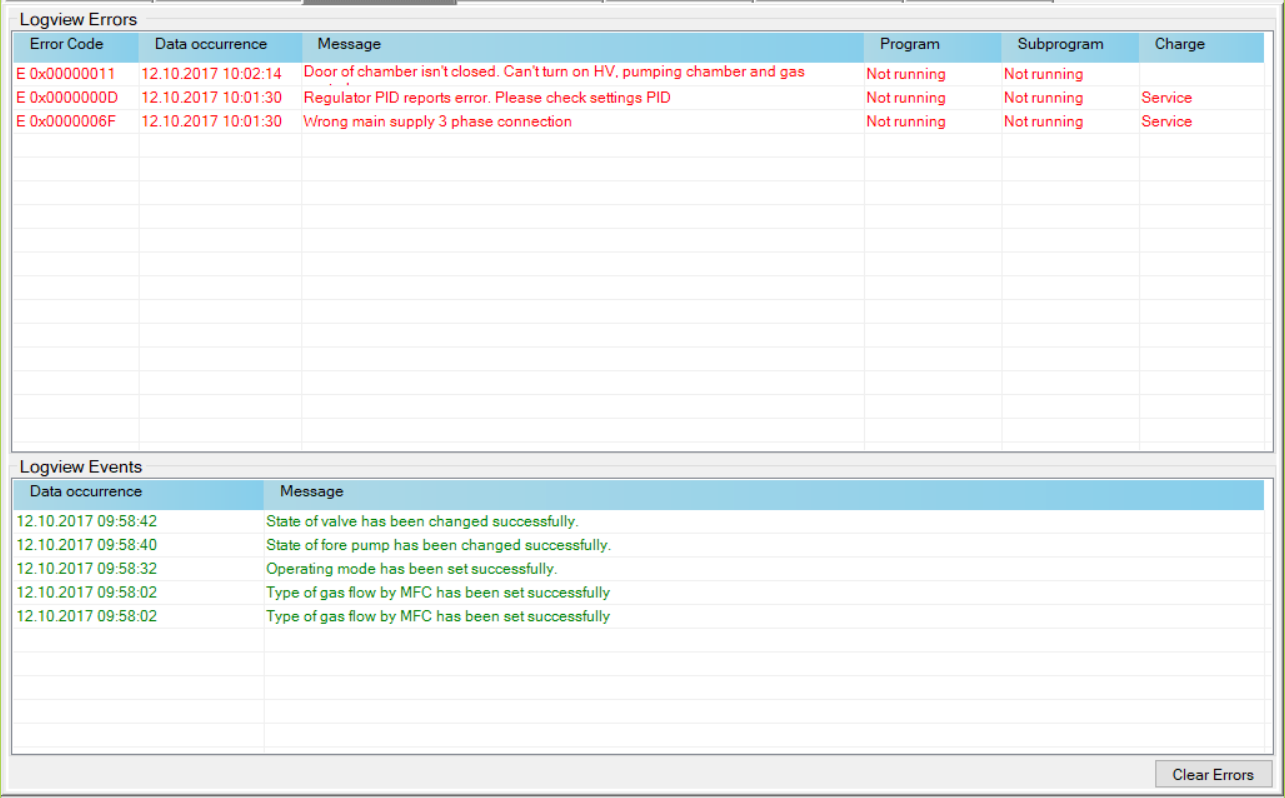
\includegraphics[width=0.7\textwidth]{Graphic/Alerts/AlertsWindow.png}	
	\caption{Alerts window}
	\label{alerts_window}
	\end{figure}
	\FloatBarrier
